\subsection{Анализ существующих аналогов}
\label{sec:analysis:analogues}

Целью данной курсовой работы является проектирование и разработка веб-сервиса для компоновки пользовательского интерфейса. 
Данное программное средство является интегрируемым сервисом, которое может использоваться как самими разработчиками для создания пользовательского интерфейса веб-приложения, так и пользователями этого веб-приложения для конфигурации пользовательского интерфейса согласно собственным предпочтениям.
Программные средства такого рода называются конструкторами сайтов или CMS и обладают следующим функционалом:

\begin{itemize}
  \item предоставление полностью готовых шаблонов сайтов с готовым дизайном;
  \item предоставление готовых дизайнерских решений для пользовательского интерфейса;
  \item гибкая система управления сайтом.
\end{itemize}

Такие сервисы целесообразно использовать для:
\begin{itemize}
  \item создания одностраничных приложеий или SPA под трафик с контекстной и таргетированной рекламой;
  \item визуализации идеи, чтобы впоследствии предоставить ее разработчикам и/или дизайнерам;
  \item быстрого запуска несложных проектов;
  \item тестирования идеи, чтобы понять, стоит ли тратить время и деньги на разработку;
  \item быстрого запуска несложных проектов;
  \item некоммерческих сайтов "для души".
\end{itemize}	

Серьезные веб-проекты лучше создавать на зарекомендовавших себя CMS или "самописных" движках, заточенных под конкретные задачи. Это так, но в некоторых ситуациях такой подход слишком долог, дорог и трудозатратен. С тем же WordPress нужно разбираться несколько недель. Если есть время и желание изучать тонкости самостоятельно или средства для оплаты услуг специалиста - отлично. В противном случае можно воспользоваться визуальными конструкторами. Это не панацея, есть проекты, которые невозможно реализовать без участия дизайнеров и программистов.
Выбирать конструктор стоит исходя из конкретных задач. Некоторые отлично справляются с Landing Page, другие - подходят для создания многостраничных сайтов, третьи хорошо продвигаются в поиске. Давайте сравним популярные сервисы, чтобы понять в какой ситуации лучше использовать тот или иной продукт.
При выборе инструмента для создания сайта нужно учитывать много параметров. Они зависят от типа ресурса и задач, которые он должен решать. Для удобства я составила сравнительную таблицу. В ней прописаны важные, на мой взгляд, характеристики и функциональные особенности конструкторов, которые упомянуты в этом обзоре.
Сравним сервисы по таким параметрам:

\begin{itemize}
  \item типы сайтов - на какие ресурсы рассчитан функционал (визитка, лендинг, магазин и т.д.);
  \item уровень пользователей - опыт в разработке: новички, продвинутые пользователи, профессионалы;
  \item адаптивность шаблонов - наличие в каталоге макетов, адаптированных для мобильных устройств;
  \item количество готовых шаблонов - сколько в каталоге готовых макетов, за которые не придется платить отдельно;
  \item уровень пользователей - опыт в разработке: новички, продвинутые пользователи, профессионалы;
  \item адаптивность шаблонов - наличие в каталоге макетов, адаптированных для мобильных устройств;
  \item количество готовых шаблонов - сколько в каталоге готовых макетов, за которые не придется платить отдельно;
  \item уровень кастомизации шаблонов - возможность изменения элементов и дизайна в целом: высокая, средняя, низкая;
  \item возможность создать сайт с нуля - можно ли открыть пустой макет и собрать страницы из блоков и виджетов;
  \item обучающие материалы - информационная база по пользованию конструктором;
  \item возможность редактировать и добавлять код - добавлять свои элементы и редактировать стили через HTML и CSS;
  \item бесплатный тариф - наличие бесплатного тарифа. Ограничения прописаны в детальном обзоре каждого конструктора ниже;
  \item триал - наличие тестового периода с расширенным функционалом.
  \item техподдержка - язык и способы поддержки пользователей;
  \item минимальный тариф - стоимость минимального тарифа;
  \item способы оплаты - варианты оплаты тарифов и дополнительных услуг;
  \item интеграции - подключение к сторонним сервисам для расширения функционала сайта;
  \item домен - возможность подключить свой домен на бесплатном тарифе, а также условия, на которых он предоставляется бесплатно;
  \item SEO - возможности оптимизации сайта;
  \item импорт/экспорт товаров - способы загрузки большого количества товаров в каталог;
  \item интеграция с CRM - подключение к CRM для автоматического импорта заказов с сайта;
  \item интеграция с системами аналитики - возможность подключиться к сторонним сервисам аналитики;
  \item онлайн-оплата - платежные системы, которые можно подключить к сайту;
  \item интеграция с соцсетями - кнопки, виджеты и комментарии.
\end{itemize}

В качестве рассматриваемых аналогов будут выступать следующие решения:
\begin{itemize}
  \item Tilda Publishing;
  \item LPgeneratorWIX.
\end{itemize}

\subsubsection{Tilda Publishing}
\

Tilda – интуитивный конструктор сайтов. Подходит для создания небольших проектов - информационных и корпоративных ресурсов, Landing Page и интернет-магазинов с десятком-другим позиций. Хотя для последних есть более удобные решения, за последний год Tilda добавила множество возможностей для этого типа сайтов. Появились полноценная корзина с вариантами доставки и оплаты, блоки карточек товаров со встроенными попапами, в которых отображаются увеличенные фотографии и расширенное описание, лейблы "хит", акция и другие для визуального выделения товаров. Кроме того, сайт интегрируется с несколькими платежными системами, интернет-эквайерами и CRM. Заявки можно отслеживать во встроенном инструменте конструктора, экспортировать в Google Sheets или Telegram.

Функционал Tilda ориентирован на эффектное оформление лонгридов - стильная типографика, много блоков для комбинирования текстового, визуального и видео-контента. Возможности не ограничиваются готовыми шаблонами и блоками - и то, и другое можно разработать самостоятельно с нуля, используя конструкторы. Для тех, у кого на это нет времени и желания, в каталоге около 200 дизайнов, которые можно настроить под себя с помощью 450 блоков. Есть готовые макеты для пиццерий, антикафе, салонов красоты и других ниш. Для визуализации отдельных элементов сайта дизайнеры Тильды отрисовали целую библиотеку иконок под разные сферы бизнеса, которая регулярно пополняется.

\pagebreak

\begin{figure}
\centering
	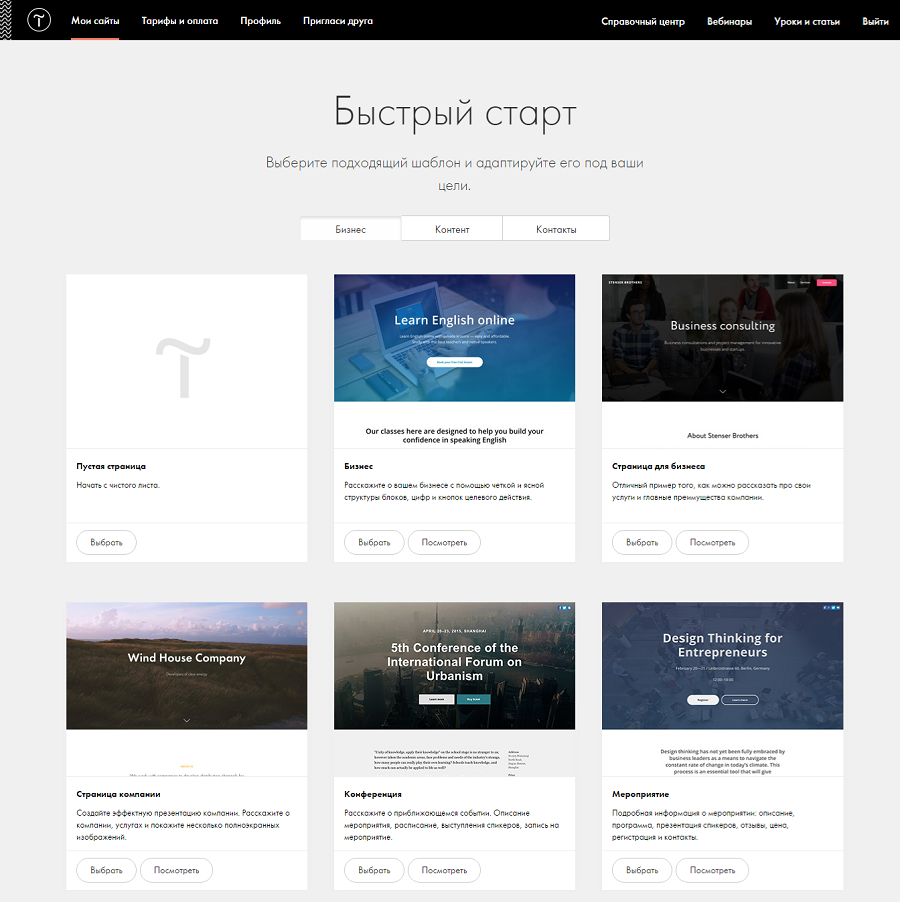
\includegraphics[scale=0.6]{tilda.png}
	\caption{Скриншот приложения "Tilda Publishing"}
	\label{sec:analysis:tilda}
\end{figure}

Достоинства:

\begin{itemize}
	\item	Большой выбор готовых шаблонов;
	\item	Удобный интуитивно понятный интерфейс;
	\item	Широкие возможности для кастомизации - цвета, шрифты, отступы, прозрачность, анимация;
	\item	Стильные адаптивные шаблоны;
	\item	Возможность отдельно настроить отступы для мобильных и десктопных версий;
	\item	Возможность создать свой уникальный макет с нуля;
	\item	Большой выбор модулей - текст, блоки преимуществ, формы заявок и обратной связи, опросов, онлайн-бронирования и т. д;
	\item	Генератор UTM-меток;
	\item	Обучающие статьи и видео-уроки по работе с сервисом;
	\item	Хорошая типографика, можно подключать шрифты из Google Fonts, Typekit и собственной коллекции;
	\item	Возможность добавить свои элементы с помощью HTML, CSS и JS;
	\item	Интеграция с CRM, сервисами обратных звонков, онлайн-чатами и электронными платежными системами;
	\item	Сайт можно перенести на другой хостинг или собственный сервер, а также интегрировать созданные на Tilda страницы с проектами на Битрикс, WordPress и другими;
	\item	Встроенная аналитика, подключение Google Analytics и <<Яндекс.Метрики>>;
	\item	Отслеживание количества кликов по кнопкам, заполнения форм и других событий в "Метрике" и "Аналитике" по умолчанию, без настройки целей;
	\item	Подключение на сайт ленты постов Instagram с автоматическим обновлением;
	\item	Возможность настроить передачу данных в налоговую в соответствии с 54-ФЗ;
	\item	Конструктор политики обработки персональных данных.
	\item	Возможность сохранить и использовать для дальнейшей работы собственные шаблоны;
	\item	Подключение HTTPS в интерфейсе конструктора.
	\item	Функционал мультилендинга - можно создать динамический контент, чтобы внешний вид сайта и информация подстраивались под конкретного пользователя;
	\item	Интеграция с популярными онлайн-банками - "Сбербанк", "Альфа Банк" и "Тинькофф", чтобы принимать платежи и получать деньги на расчетный счет;
	\item	Функционал для верстки email-рассылок с последующей отправкой через MailChimp, UniSender или любой другой сервис с помощью экспорта кода.
\end{itemize}

Недостатки:

\begin{itemize}
	\item Высокие тарифы;
	\item Для хорошего результата требуются определенные познания в веб-дизайне.
\end{itemize}

\subsubsection{LPgenerator}
\

LPgenerator – мощный сервис для разработки одностраничных сайтов. Узкая специализация с лихвой окупается множеством возможностей и интеграций. Не подойдет для создания визитки, блога, информационного портала или онлайн-гипермаркета. Есть возможность подключить на одностраничник витрину, но этот инструмент скорее дополнительный. Зато лендинг при должных навыках получится что надо. 
Сервис ориентирован на профессионалов. Разработчики заинтересованы в том, чтобы на их платформе создавались красивые и конверсионные сайты. Об этом говорит все - от стоимости и содержания тарифов до уровня тех. поддержки и обучения новых пользователей. В LPG есть все для создания уникальных профессиональных сайтов - множество красивых современных шаблонов вкупе с широкими возможностями кастомизации, сборка макета из блоков с чистого листа и доступ к HTML/CSS коду. Но главное отличие от других конструкторов заключается в дополнительных инструментах для раскрутки и заработка на лендингах - CRM и работа с лидами, подробная и детальная аналитика, управление источниками трафика и многое другое.

\begin{figure}
\centering
	\includegraphics[scale=0.6]{lpgenerator.png}
	\caption{Каталог шаблонов "LPgenerator"}
	\label{sec:analysis:lpgenerator}
\end{figure}